
\subsection{Recommended Implementation}
\begin{itemize}
    \item \textbf{Web Application}: the web application should be written in a web framework such as \emph{Vue.js} or \emph{Angular} to create a consistent web interface with cross platform support.
    \item \textbf{Application Server}: the recommended implementation for the server uses the \emph{Rust} language, the \emph{Actix}\footnote{\href{https://actix.rs/}{https://actix.rs/}} actor framework and \emph{SQLx}\footnote{\href{https://github.com/launchbadge/sqlx}{https://github.com/launchbadge/sqlx}}. The Rust language provides a safe, concurrent alternative over C and C++ while providing comparable performance, allowing high reliability and throughput for the service.
    \item \textbf{In-Memory data store}: the in memory data store employed may be \emph{Redis Enterprise}
    \item \textbf{DBMS}: the relational database manager software may be \emph{PostgreSQL 13}
    \item \textbf{Reverse Proxy}: the reverse proxy may be \emph{NGINX}
\end{itemize}

\subsection{Implementation Plan}

The implementation should follow a \emph{Thread} (also known as \emph{Tracer bullet}\cite{pragmatic}) approach. 

\begin{figure}[H]
    \centering
    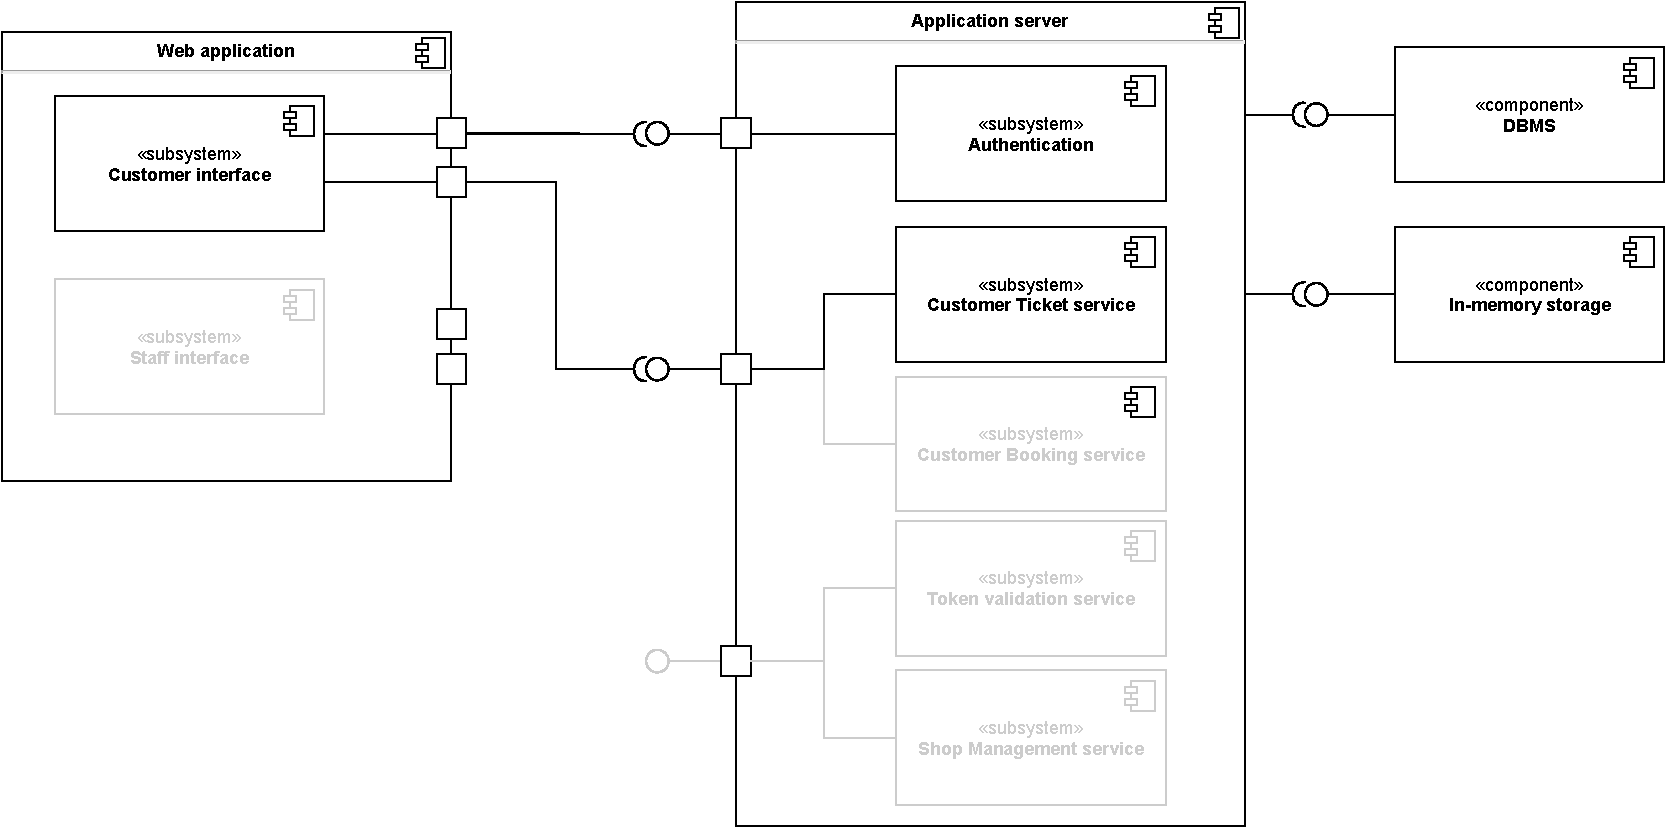
\includegraphics[width=0.9\textwidth]{Images/component2_tb.pdf}
\end{figure}

The system should be written starting from a subset of functionality implemented from the start to the end. Then the other functionalities will be added alongside what was already written.

The first thing to be programmed should be the authentication and account creation, interfacing with the DBMS and the memory storage and exposing a minimal API.

This way, the system can reach partial functionality with a structure representative of the final product in a small amount of time. Then other components can rely on the existing structure for integration.

The Ticket service should be implemented and integrated right after the Authentication, adding part of the core functionality.

The web application can be developed in parallel by referencing the proposed REST API for the first stages of development.

At this point a partially working version of the system is complete and can be presented to the stakeholders for feedback.

The next components should be created and integrated in the following order:
\begin{itemize}\tightlist
    \item Staff interface, with the associated Token Validation service
    \item Booking service
    \item Shop management service
\end{itemize}

The Search engine and Maps service  interfaces can be added in parallel after the first working version, since they have essentially zero coupling to the other parts of the system.

\subsection{Testing plan}

Testing should be done throughout all stages of development, following a bottom up approach.

Unit tests should be written starting from the basic component so that tests for other components that use them can be written relying on the fact that the subcomponents are already tested. This speeds up debugging since it's easy to locate at which level of the component hierarchy there is a problem.

Tests for the application server which interact with the database should be run on an indipendent instance of the service and not on the main network.

\subsection{Integration plan}
The main branch of the version control should be reserved for working and potentially deliverable, versions of the system. The web application and the application server should have two separate repositories, in order to make the commit history more readable. \emph{Feature branches} should be created as necessary, to work on adding new features to the system.

Testing should be enforced through a \emph{Continuous Integration} platform such as GitLab CI, Travis CI or GitHub Actions. This way every commit will be tested and marked, so that broken commits will be highlighed and will not be merged into the main branch.